\appendix
\chapter{User Manual}




\section{Preface: A user manual for a mobile app? Are you kidding me?}

Although many app developers and phone manufacturers think that there is no need to provide a user manual for a mobile app (they think users ``enjoy'' discovering hidden features) we feel it is better for the user to be able to understand how any software works. Therefore, you don't have to look if the app can do something or not. You just check the manual. So, if you are looking forthe way to do something and it is not in this manual... it probably cannot be done :-) .




\section{Starting the Application}

Once installed you can launch the application from your apps menu in your phone. The loading screen (figure \ref{fig:initScreen}) will appear showing the name of the program and its version number.


\begin{figure}
 \centering
 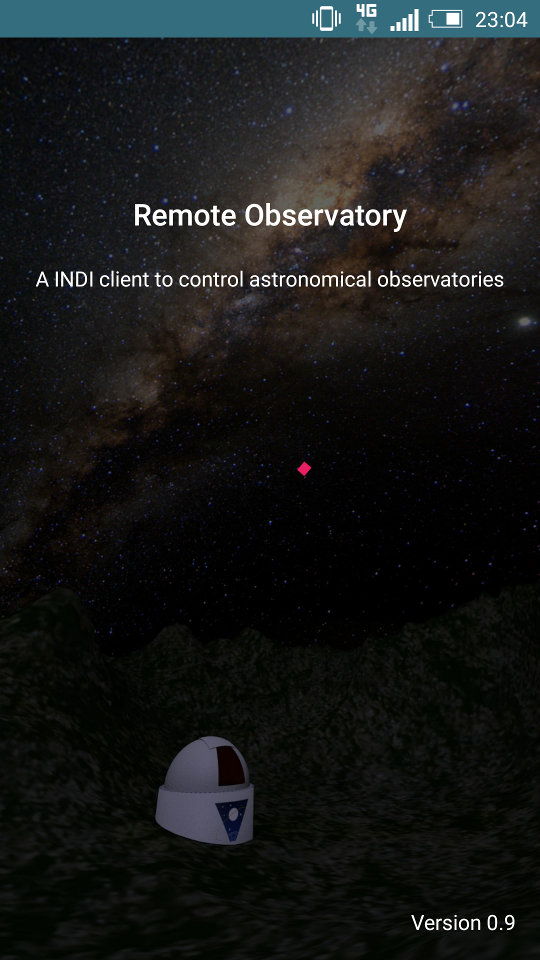
\includegraphics[width=5cm]{../images/initScreen.jpg}
 \caption{Init Screen}
 \label{fig:initScreen}
\end{figure}




            

\section{Main Screen Description}

The main screen is divided in three main regions (image \ref{fig:mainScreen}):

\begin{itemize}
  \item \textbf{Top Button Bar:} From where you can access to the \texttt{Connection / Device selection}  
\includegraphics[width=0.5cm]{../images/connectionDeviceSelectionButton.png}, the \texttt{Add Connection}  
\includegraphics[width=0.5cm]{../images/addConnectionButton.png} and \texttt{Main Menu} 
\includegraphics[width=0.5cm]{../images/mainMenuButton.png} buttons. These will be described in more detail in the following.
  \item \textbf{Tabs Bar:} In this bar you will be able to select the different interfaces for each of the INDI devices that you are connected to.
  \item \textbf{Main Control:} The main portion of the app is dedicated show the different properties of the INDI devices. At this point, this part of the screen just shows some general help about the app.
\end{itemize}


\begin{figure}
 \centering
 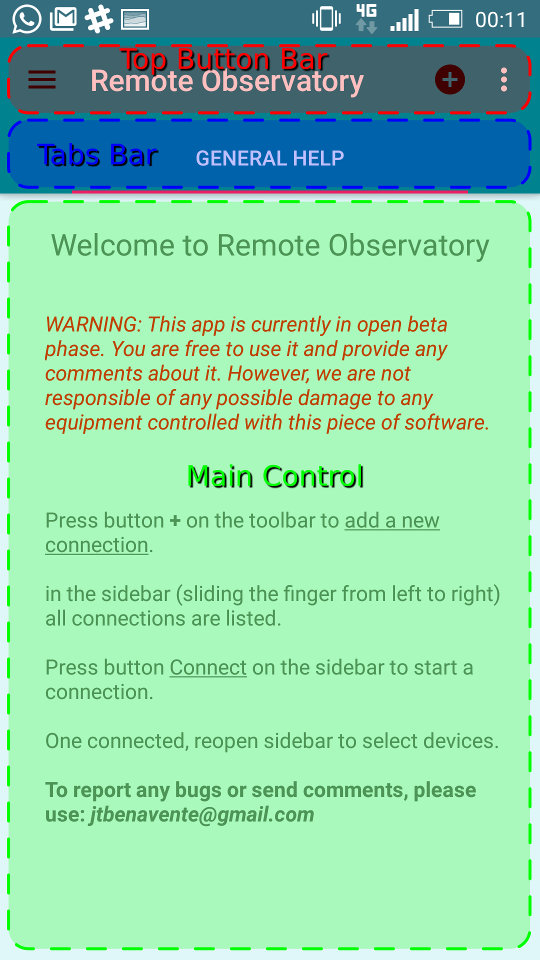
\includegraphics[width=5cm]{../images/mainScreen2.jpg}
 \caption{Main Screen}
 \label{fig:mainScreen}
\end{figure}

                
                

\label{manageConnections}
\section{Managing Connections}

To control any INDI device you must connect to the server it is plugged in. To do so, \textbf{Remote Observatory} allows you to define one or more INDI servers (connections) to which you can connect. The first step to add a connection is to press the \texttt{Add Connection} 
\includegraphics[width=0.5cm]{../images/addConnectionButton.png} button. A form will appear (figure \ref{fig:newConnection}) in which several fields are required:

\begin{enumerate}
  \item \texttt{Name}: A name for the connection (just to identify it) \textit{Example: \texttt{My Observatory}}.
  \item \texttt{Server}: The IP address or domain of your INDI Server. \textit{Examples: \texttt{198.51.100.3} or \texttt{indi.example.com}}.
  \item \texttt{Port}: The port of your INDI server. Typically 7624, but it depends on your server configration. \textit{Example: \texttt{7624}}.
  \item \texttt{Autoconnect}: Enabling it will make the app to connect to the server when starting.
  \item \texttt{Enable BLOBs}: The app will ask the server to send \texttt{BLOB} data. This is for example important if you pretend to get images from a CCD. Please note that \texttt{BLOBs} often sends quite big amounts of data (not good if you have restrictions on your mobile data connection).
\end{enumerate}

Once you \texttt{Add} the connection it will appear in the \texttt{Connection / Device selection} panel (figure \ref{fig:connectionAndDevicesPanel}), accesible from its button in the top button bar. From that panel you can \texttt{Edit} any of the fields of the connection or \texttt{Connect} to the server. Finally, if you want to delete a connection that will be no longer in use, you can use the \texttt{Remove Connections} option in the \texttt{Gereral Options} menu.


\begin{figure}
 \centering
 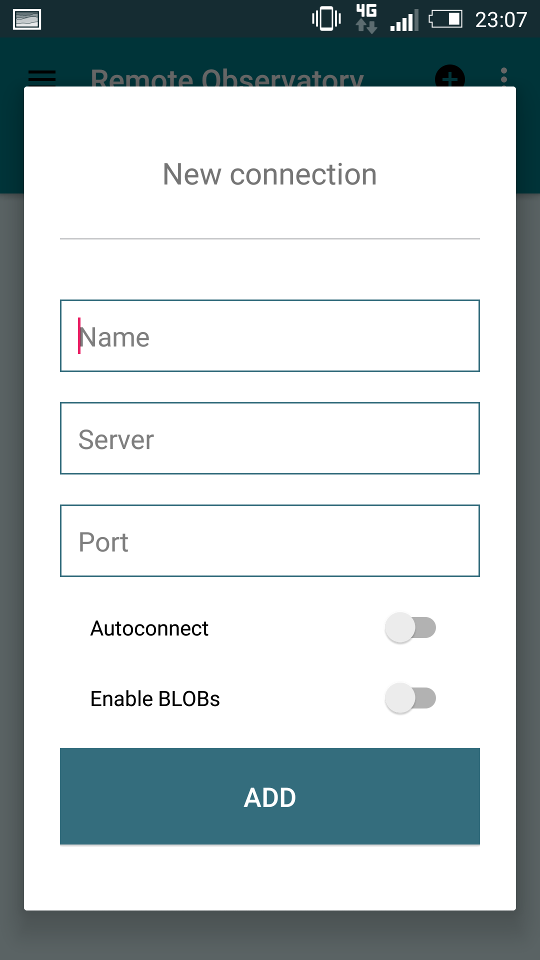
\includegraphics[width=5cm]{../images/newConnection2.png}
 \caption{New Connection}
 \label{fig:newConnection}
\end{figure}


\begin{figure}
 \centering
 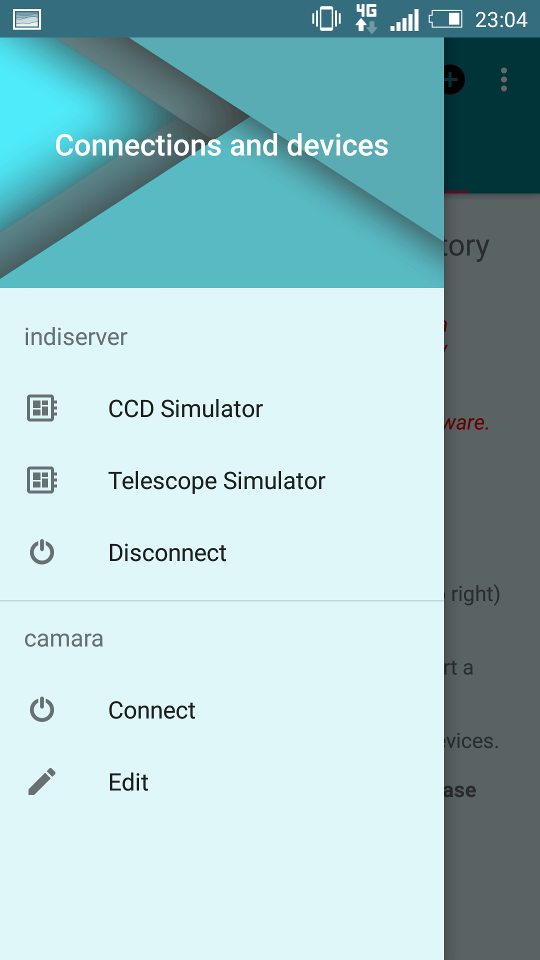
\includegraphics[width=5cm]{../images/connectionAndDevicesPanel2.png}
 \caption{Connection and Devices Panel}
 \label{fig:connectionAndDevicesPanel}
\end{figure}


            

                
\label{settings}
\section{Adjusting Settings}

There are several configuration options that control the general behaviour of the app. You can find those options under the \texttt{Settings} (figure \ref{fig:mainMenu}) option in the \texttt{Main Menu} 
\includegraphics[width=0.5cm]{../images/mainMenuButton.png} (figure \ref{fig:settings}):

\begin{itemize}
  \item \texttt{Notifications}: The app can be configured to alert of some conditions (new devices found, connections that are lost, etc) using different mechanisms:
  
  \begin{itemize}
    \item \texttt{System Notifications}: Using system notifications, usually visible in the upper menu in your android device.
    \item \texttt{Dialog Notifications}: Using a dialog that shows the appropriate message.
    \item \texttt{Sound Notifications}: A sound will be played.
    \item \texttt{Vibrate Notifications}: The phone will vibrate.
  \end{itemize}
  
  
  \item \texttt{General Settings}:
  \begin{itemize}
    \item \texttt{Default Folder}: The default folder in which configuration files and \texttt{BLOB} data will be saved.
  \end{itemize}
  

\end{itemize}


\begin{figure}
 \centering
 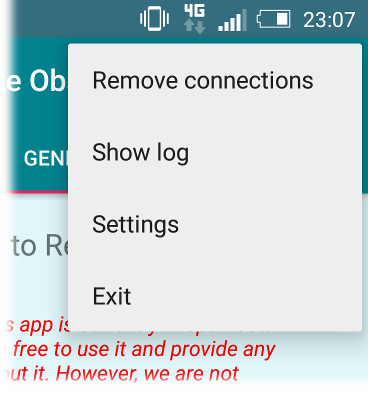
\includegraphics[width=5cm]{../images/mainMenu2.png}
 \caption{Main Menu}
 \label{fig:mainMenu}
\end{figure}

\begin{figure}
 \centering
 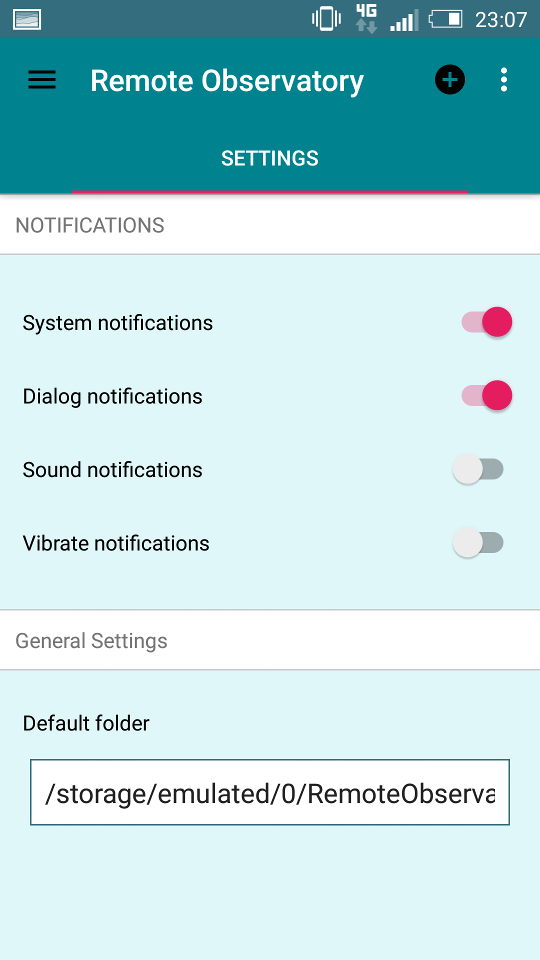
\includegraphics[width=5cm]{../images/settings2.png}
 \caption{Settings}
 \label{fig:settings}
\end{figure}


   

\section{Logging}

All the activity from / to de different devices are logged in text files which are accesible to the user. This logs may help the user to detect any problem or understand what has happened during an abservation session. Each connection has an associated log file:

\begin{itemize}
  \item \textbf{To view the logs} just use the \texttt{Show log} option in the \texttt{Main Menu} 
\includegraphics[width=0.5cm]{../images/mainMenuButton.png} (figure \ref{fig:viewLog}).
  
  \item \textbf{To Clear a file log} use the \texttt{Remove log} option in the \texttt{Edit} panel for the connection (figure \ref{fig:editConnection}).
\end{itemize}


\begin{figure}
 \centering
 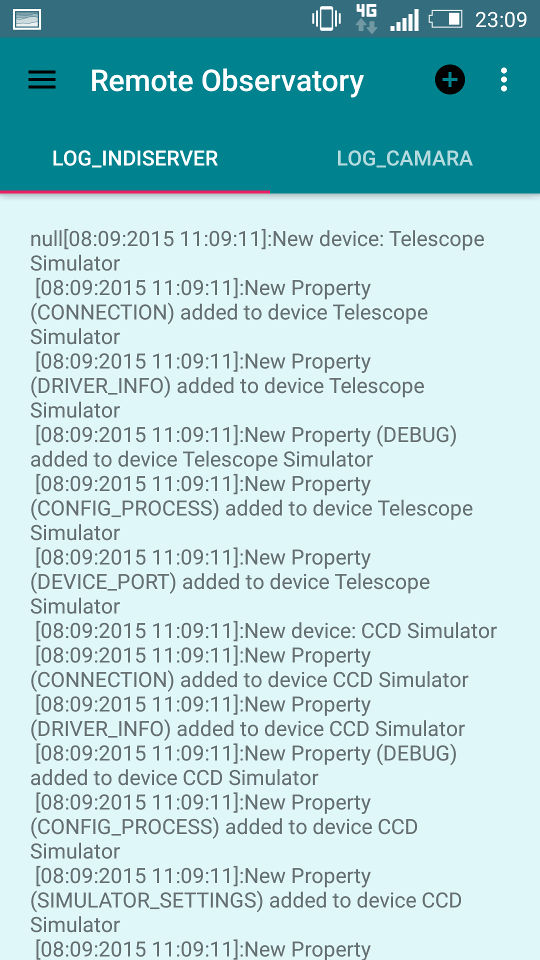
\includegraphics[width=5cm]{../images/log2.jpg}
 \caption{View Log}
 \label{fig:viewLog}
\end{figure}

\begin{figure}
 \centering
 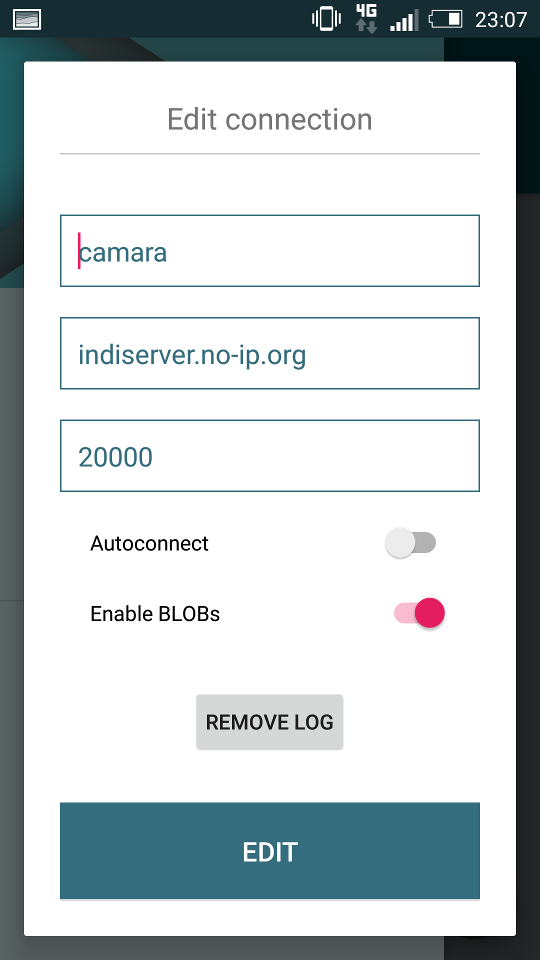
\includegraphics[width=5cm]{../images/editConnection2.png}
 \caption{Edit Connection}
 \label{fig:editConnection}
\end{figure}



\section{Connecting and Disconnecting from INDI Servers}

Once you have set up at least one connection (section \ref{manageConnections}), you can connect to it by pressing the \texttt{Connect} button in the \texttt{Connection / Device selection} panel (figure \ref{fig:connectionAndDevicesPanel}). Once the connection is established the app may recieve information about all the devices in that INDI server.

To disconnect from a particular INDI server, just use the \texttt{Disconnect} button in the \texttt{Connection / Device selection} panel. Please note that if for any reason the connection is lost (the mobile phone losts its connection, the server is restarted, etc.), the app will notify us about this situation by means of any activated controls in the Settings (section \ref{manageConnections}) (vibration, sound, system notification and/or dialog).



\begin{figure}
 \centering
 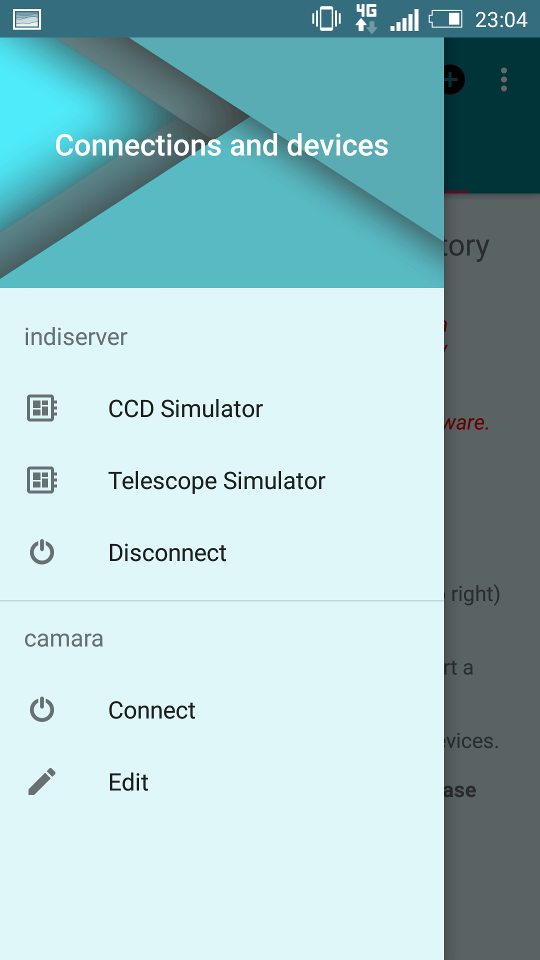
\includegraphics[width=5cm]{../images/connectionAndDevicesPanel2.png}
 \caption{Connect Button}
 \label{fig:connectButton}
\end{figure}




\section{Device Views}

Once a connection is established the server will usually send the available devices. To check the properties of any device, you can again click on the \texttt{Device Name} in the \texttt{Connection / Device selection} panel. This action will add at least a new tab to the \texttt{Tabs Bar} with the name of the device. Please take into account that to ease the management of different devices, more than one view for a particular device might be added to the \texttt{Tabs Bar}.

The \texttt{Default Device View} \ref{fig:defaultView}) consists on a list of INDI Properties that are grouped according to their nature in different  dropdown lists. Each property value, status and information is updated whenever the server send any change about it. Each property has some common icons on its left side:


\begin{figure}
 \centering
 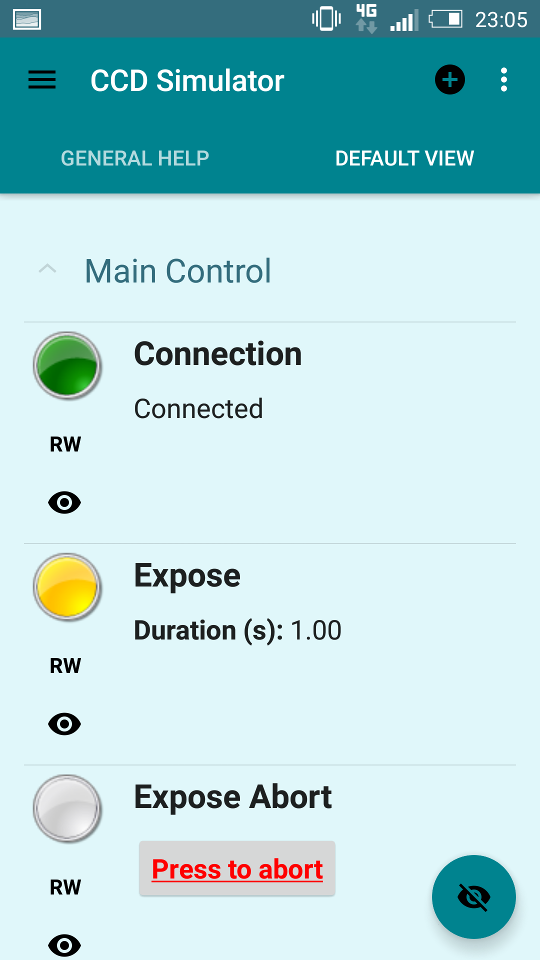
\includegraphics[width=5cm]{../images/defaultView.png}
 \caption{Default Device View}
 \label{fig:defaultView}
\end{figure}




\begin{itemize}
  \item \texttt{Property State Icon}: INDI properties must have one state. Each state is represented by a icon with the following colors: 
    \begin{itemize}
      \item \textbf{Idle:} Gray 
\includegraphics[width=0.5cm]{../images/grey_light_32.png} (the property has not yet been set).
      \item \textbf{Ok:} Green 
\includegraphics[width=0.5cm]{../images/green_light_32.png} (the value of the property is correct).
      \item \textbf{Busy:} 
\includegraphics[width=0.5cm]{../images/yellow_light_32.png} Yellow (the property is adjusting its value).
      \item \textbf{Alert:} 
\includegraphics[width=0.5cm]{../images/red_light_32.png} Red (there was some problem with the property value).
    \end{itemize}
  
  
  \item \texttt{Property Permission}: INDI properties must show any of the following permissions:
    \begin{itemize}
      \item \textbf{Read / Write:} Denoted by a \texttt{RW} icon. The property values can be read and written.
      \item \textbf{Read Only:} Denoted by a \texttt{RO} icon. The property values can be read, but not written.
      \item \textbf{Write Only:} Denoted by a \texttt{WO} icon. The property values can be written, but not read.
    \end{itemize}
  
  
  \item \texttt{Visibility Icon} 
\includegraphics[width=0.5cm]{../images/visibility1.png} 
\includegraphics[width=0.5cm]{../images/visibility2.png}: Which allow to show / hide particular properties. Please check hidding / showing properties (section \ref{hidding}).
\end{itemize}

               
On the right of those icons the app shows the current values for each one of the elements of the property. Depending on the nature of the property a slightly different interface is used to show that information:



\begin{itemize}
  \item \textbf{Text properties:} It just shows the text value of each element of the property.
  \item \textbf{Number properties:} It shows the number value of each element of the property, formatted in its appropriate way (integer, float, sexagesimal...).
  \item \textbf{Light properties:} It shows an icon representing the light state:
    \begin{itemize}
      \item \textbf{Idle:} Gray 
\includegraphics[width=0.5cm]{../images/grey_light_32.png}.
      \item \textbf{Ok:} Green 
\includegraphics[width=0.5cm]{../images/green_light_32.png}.
      \item \textbf{Busy:} Yellow 
\includegraphics[width=0.5cm]{../images/yellow_light_32.png}.
      \item \textbf{Alert:} Red 
\includegraphics[width=0.5cm]{../images/red_light_32.png}.
    \end{itemize}
  
  \item \textbf{Switch properties:} It will show which of the options on the switch are \texttt{ON} or \texttt{OFF}.
  \item \textbf{BLOB properties:} It will show the size of the \texttt{BLOB} packet (in bytes), its type (usually a file extension) and a pair of buttons:
    \begin{itemize}
      \item \texttt{Save button} 
\includegraphics[width=0.5cm]{../images/saveBlobButton.png}: It will save the \texttt{BLOB} data to the appropriate folder (see section \ref{settings}). 
      \item \texttt{Preview button} 
\includegraphics[width=0.5cm]{../images/viewBlobButton.png}: It will launch another application on the phone that is able to manage the \texttt{BLOB}. Please note that if you want to visualize \texttt{.fits} images an appropriate app that handles that image type should be installed in your device.
    \end{itemize}
\end{itemize}

\begin{figure}
 \centering
 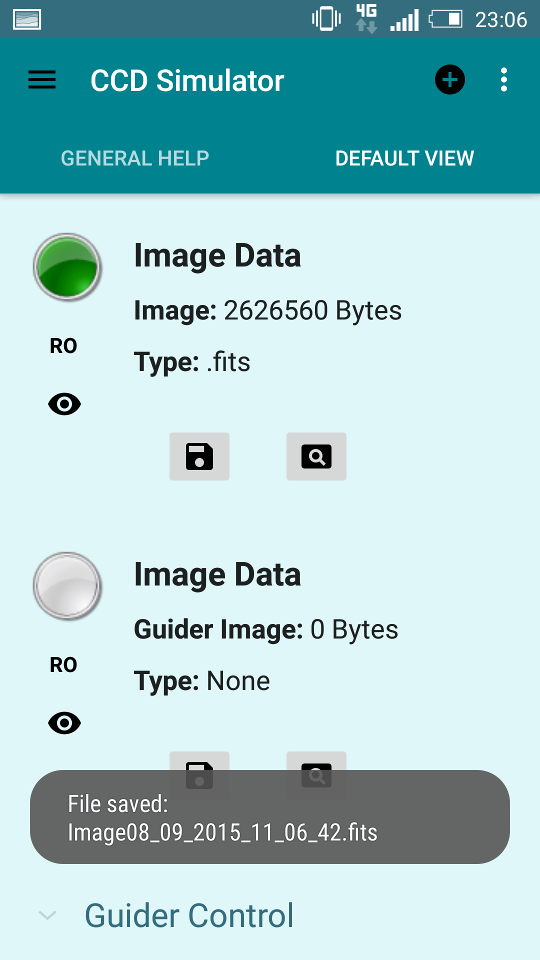
\includegraphics[width=5cm]{../images/saveBlob2.png}
 \caption{Saving Blob Data}
 \label{fig:saveBlob}
\end{figure}





\section{Updating Properties}

Every property that has a \texttt{RW} or \texttt{WO} permission can be updated with new values. To do so, you just click on the property to update. If a \texttt{RO} is clicked an alert will be shown (figure \ref{fig:readOnly}). Depending on the nature of the property a different form will be shown to update the property values:

\begin{itemize}
  \item \textbf{Text Property:} A form with the text values to change (figure \ref{fig:updateText}).
  \item \textbf{Number Property:} A form with the number values to change. The number \texttt{format} and \texttt{min} and \texttt{max} wil be shown and incorrect values will be filtered (figure \ref{fig:updateNumber}).
  \item \textbf{Switch Property:} An array of the possible selection elements will be shown. The \texttt{Switch Rule} will prevent the user to turno on more elements that are allowed (figure \ref{fig:updateSwitch}).
  \item \textbf{BLOB Property:} An interface that allows to pick files from your device to send its contents to the property.
\end{itemize}

\begin{figure}
 \centering
 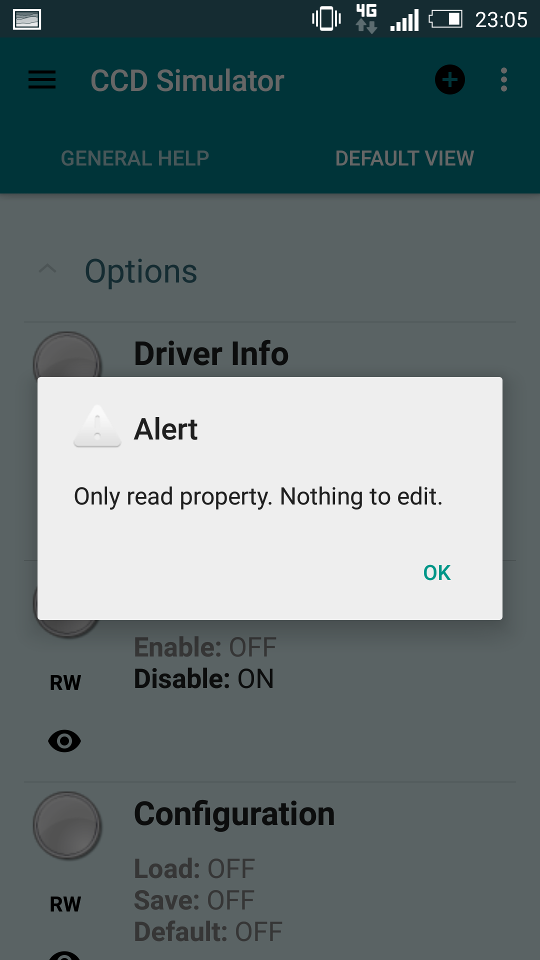
\includegraphics[width=5cm]{../images/readOnlyProperty2.png}
 \caption{Read Only Property Alert}
 \label{fig:readOnly}
\end{figure}

\begin{figure}
 \centering
 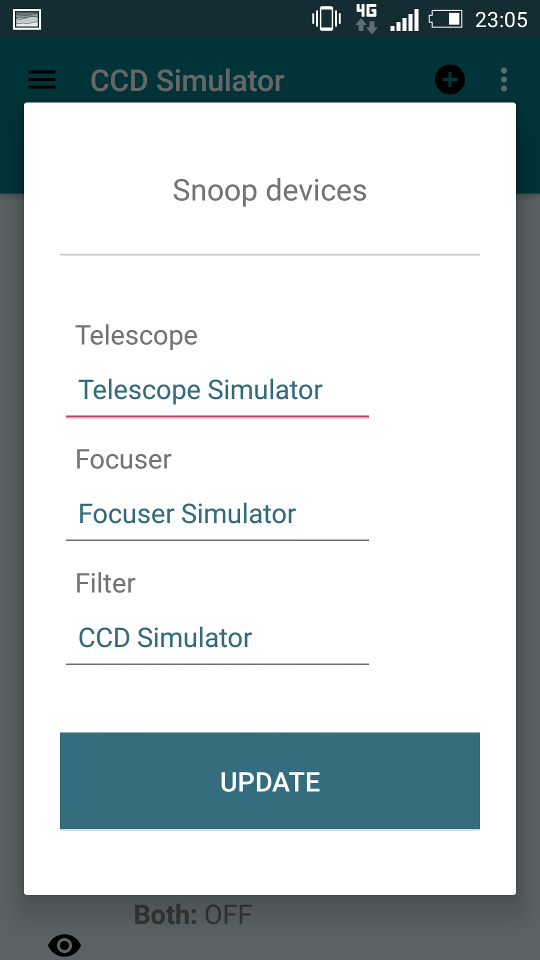
\includegraphics[width=5cm]{../images/updateText2.png}
 \caption{Updating a Text Property}
 \label{fig:updateText}
\end{figure}
                
\begin{figure}
 \centering
 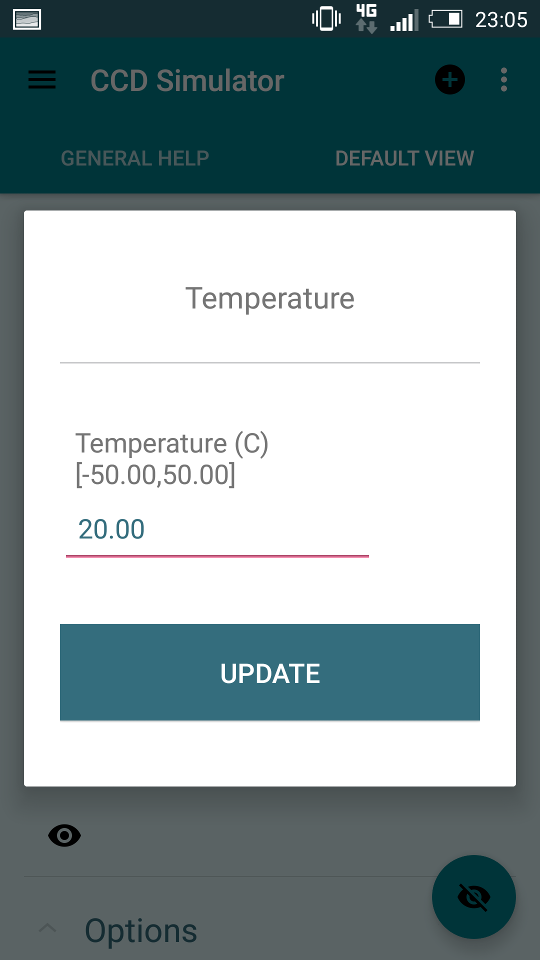
\includegraphics[width=5cm]{../images/updateNumber2.png}
 \caption{Updating a Number Property}
 \label{fig:updateNumber}
\end{figure}
                
\begin{figure}
 \centering
 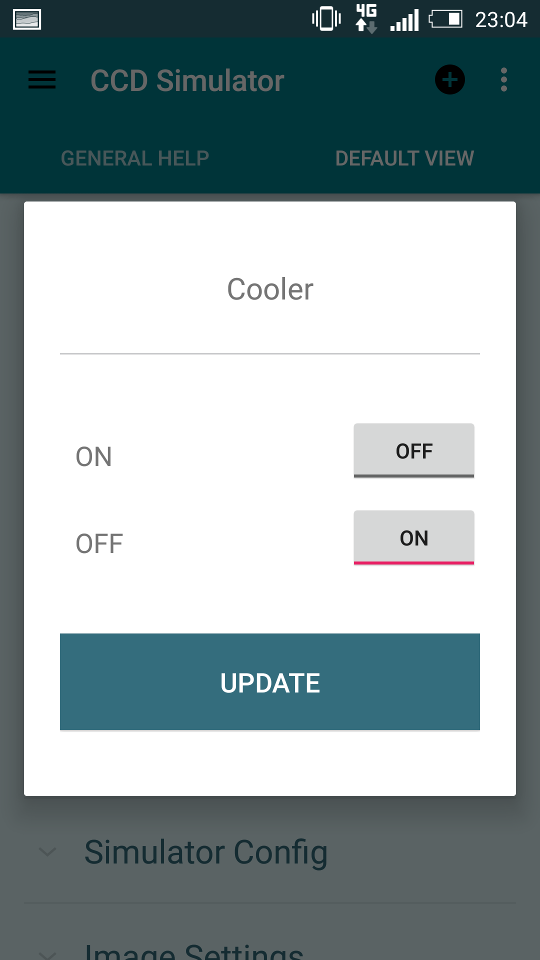
\includegraphics[width=5cm]{../images/updateSwitch2.png}
 \caption{Updating a Switch Property}
 \label{fig:updateSwitch}
\end{figure}
                

   
  

\label{hidding}
\section{Hidding / Showing Properties}

As devices usually have a large amount of properties and some of them are not used very often by the user (configration ones, for example) the \texttt{Default Device View} allows to hide them in order to simplify the interface. To do so, we can toggle the \texttt{Visibity} 
\includegraphics[width=0.5cm]{../images/visibility1.png} 
\includegraphics[width=0.5cm]{../images/visibility2.png} button on the property.

However, to be able to show a hidden property, a \texttt{Global Visibility} toggle button (figure \ref{fig:globalVisibility}) has been incorporated (visible on the lower right part of the app when scrolling). When that button is 
\includegraphics[width=0.5cm]{../images/visibility1.png}, all properties will be shown. When it is 
\includegraphics[width=0.5cm]{../images/visibility2.png} only the properties with its \texttt{Visibility} button 
\includegraphics[width=0.5cm]{../images/visibility1.png} will be shown.

\begin{figure}
 \centering
 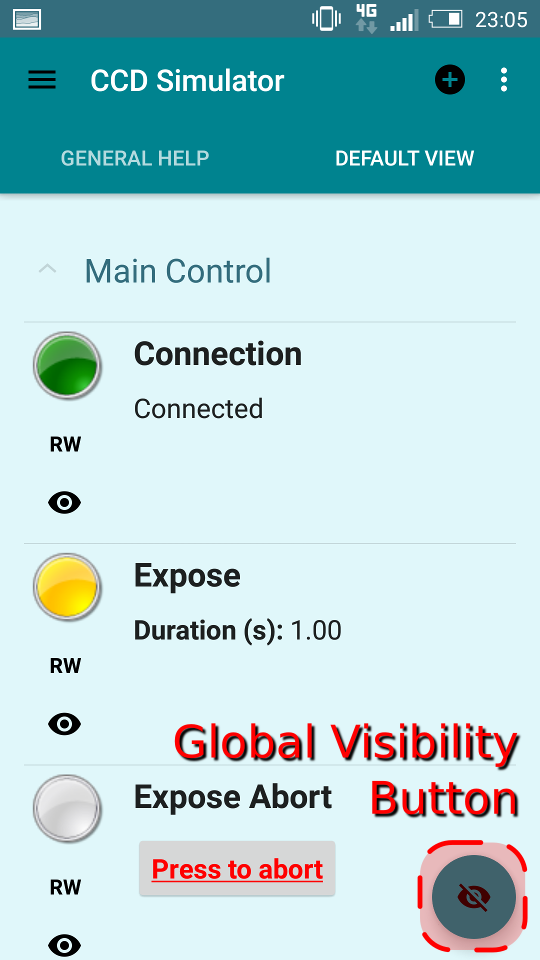
\includegraphics[width=5cm]{../images/globalVisibility.png}
 \caption{Global Visibility Button}
 \label{fig:globalVisibility}
\end{figure}
